\documentclass[journal]{./IEEE/IEEEtran}
\usepackage{cite,graphicx,float,listings,url}

\newcommand{\SPTITLE}{Algorithmic Approaches to Classic Strategy Games - A Comparative Analysis of Search Techniques}
\newcommand{\ADVISEEA}{Clarence Joshua T. Bernardino}
\newcommand{\ADVISEEB}{Elisha Julianne Claveria}

\newcommand{\BSCS}{Bachelor of Science in Computer Science}
\newcommand{\ICS}{Institute of Computer Science}
\newcommand{\UPLB}{University of the Philippines Los Ba\~{n}os}
\newcommand{\REMARK}{\thanks{Presented to the Faculty of the \ICS, \UPLB\
                             in partial fulfillment of the requirements
                             for the Degree of \BSCS}}
        
\markboth{CMSC 170 Introduction to Artificial Intelligence, \ICS}{}
\title{\SPTITLE}
\author{\ADVISEEA~and~\ADVISEEB%
\REMARK
}
\pubid{\copyright~2006~ICS \UPLB}

%%%%%%%%%%%%%%%%%%%%%%%%%%%%%%%%%%%%%%%%%%%%%%%%%%%%%%%%%%%%%%%%%%%%%%%%%%

\begin{document}

% TITLE
\maketitle

% SECTION 1
\section{Introduction}
Classic games such as Tic-Tac-Toe and the 8-puzzle have long served as foundational models for problem-solving and cognitive development. While traditionally associated with human recreation, these games also provide a structured and well-defined domain for evaluating the efficacy of artificial intelligence search algorithms. This paper presents a formal analysis of these canonical problems, transposing them from a human context to a computational one. We implement and systematically evaluate four fundamental search strategies, Breadth-First Search (BFS), Depth-First Search (DFS), the A* algorithm, and the Minimax decision rule, to solve and play these games autonomously. The objective of this study is to compare the performance of these algorithms in terms of completeness, optimality, time complexity, and space complexity, illustrating the practical trade-offs in automated problem-solving.

\subsection{Algorithmic comparison of BFS, DFS, A*, minimax}
What is your understanding of the algorithms based on the three exercises?

\subsection{Breadth-First Search (BFS) and Depth-First Search (DFS)}
The search algorithms can be characterized by their distinct exploration strategies. BFS and DFS are categorized as "blind" search strategies, as they traverse the board systematically without utilizing any information other than depth to guide the search toward a goal.\cite{geeksforgeeks-Uninformed-Search-Algorithms-in-AI}

\subsection{A* Search}
In contrast, the A algorithm* is an informed search method that uses a heuristic function, h(n), to guide its exploration toward the goal. It prioritizes nodes by minimizing the total estimated cost, f(n) = g(n) + h(n), where g(n) is the known path cost. This strategy is proven to be both complete and optimal, provided the heuristic never over-estimates the path-cost from any given node.\cite{geeksforgeeks-A-star-Search-Algorithm}

\subsection{Minimax Search}
For adversarial environments, the Minimax algorithm offers a strategic framework that is guaranteed to produce optimal play against a rational opponent. The algorithm recursively evaluates a game tree by propagating static evaluation scores from terminal states back to the root. A value of +1 is assigned to a win for the maximizing player, and -1 for a win for the minimizing player. The maximizing player selects moves that lead to the highest-valued states, while the minimizing player chooses moves leading to the lowest-valued states. Consequently, an agent implementing Minimax is assured of selecting the most advantageous move available in any given state.\cite{geeksforgeeks-Adversarial-Search-Algorithms-in-Artificial-Intelligence-(AI)}

% SECTION 2
\section{Methods}
The implementation of the 8-puzzle employed the DFS, BFS, and A* algorithms. By representing board states as strings and utilizing hashing via Python sets, the design ensured an efficient solution. The Tic-Tac-Toe game, on the other hand, utilized a class-based implementation to encapsulate the board state, thereby eliminating the redundancy of passing state through function parameters. This object-oriented approach provided a structured framework for implementing the Minimax algorithm, which recursively evaluates potential moves to determine the optimal strategy.

% formatting sources - 
% https://www.overleaf.com/learn/latex/Lists
% https://tex.stackexchange.com/questions/48632/underscores-in-words-text
\subsection{8-puzzle Implementation (Full Code in Appendix)}
\begin{itemize}
  \item \texttt{find\_gap(board)} – Locates the index of the blank tile ('0') within the string-encoded board state.

  \item \texttt{finished\_state(board)} – Returns True if the current board state matches the goal configuration ('123456780').

  \item \texttt{get\_possible\_moves(board)} – Determines all valid actions ('w', 'a', 'x', 'd') for the blank tile based on its grid position.

  \item \texttt{apply\_move(board, direction)} – Generates and returns a new board state by swapping the blank tile with an adjacent tile in the given direction.
\end{itemize}

\begin{itemize}
  \item \texttt{solve\_bfs(initial\_state)} – Explores the state space using a FIFO queue, guaranteeing a shortest-path solution.

  \begin{figure}[H]
    \centering
    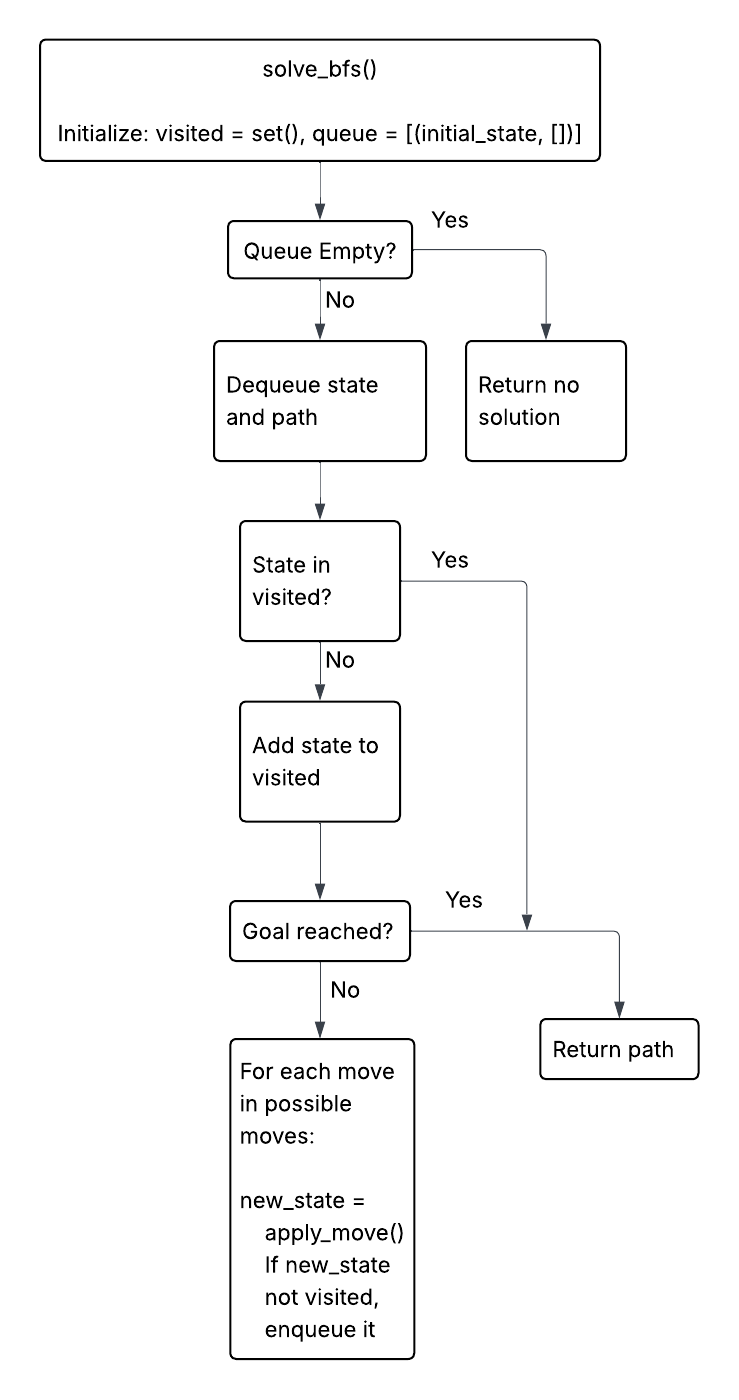
\includegraphics[width=0.6\linewidth]{pictures-Clarence/bfs flowchart.png}
    \caption{BFS Flowchart Diagram}
    \label{fig:bfs_flowchart}
\end{figure}

  \item \texttt{solve\_dfs(initial\_state)} – Explores the state space using a LIFO stack, prioritizing depth-first expansion.
  
  \begin{figure}[H]
    \centering
    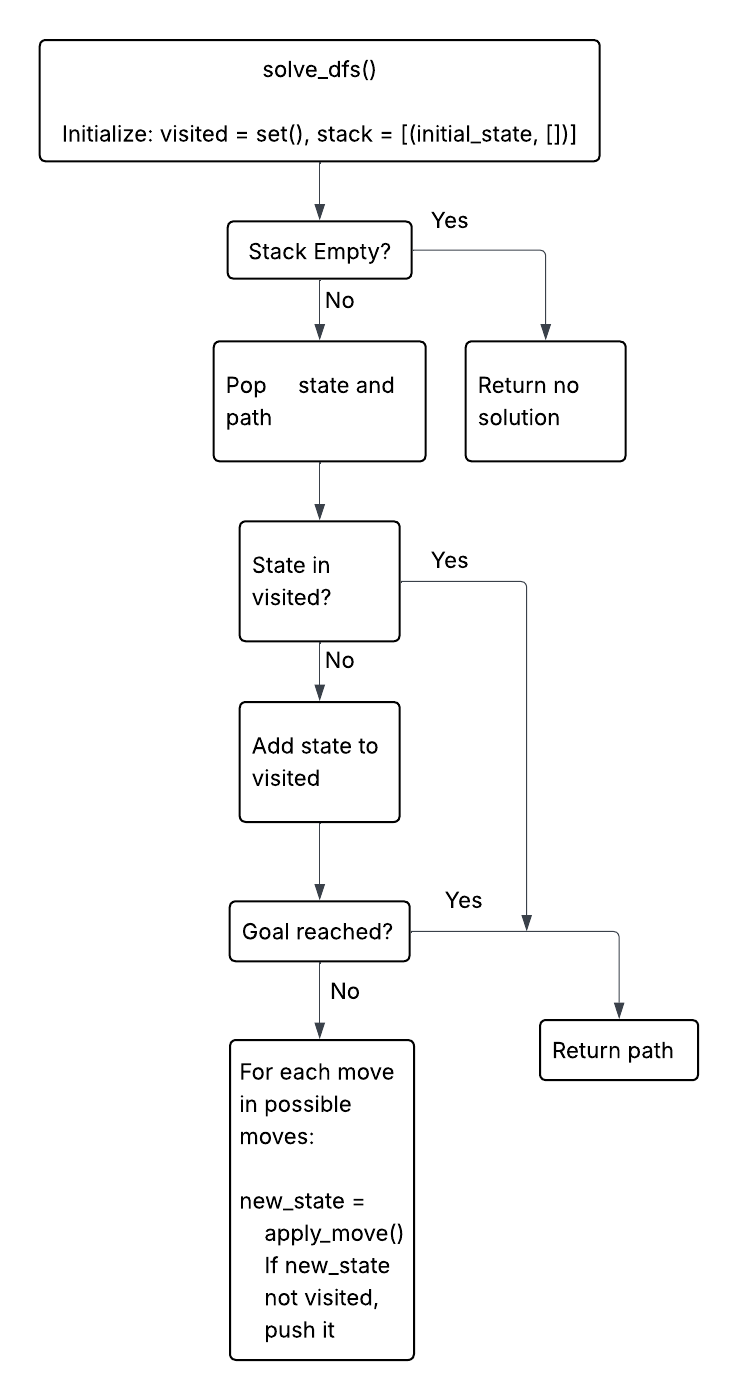
\includegraphics[width=0.6\linewidth]{pictures-Clarence/dfs flowchart.png}
    \caption{DFS Flowchart Diagram}
    \label{fig:dfs_flowchart}
  \end{figure}

  \item \texttt{heuristic\_manhattan(board)} – Computes the sum of the Manhattan distances of each tile from its goal position.

  \item \texttt{solve\_astar(initial\_state, heuristic)} – Explores states by prioritizing the lowest estimated total cost (F = path cost (G) + heuristic (H)).

  \begin{figure}[H]
    \centering
    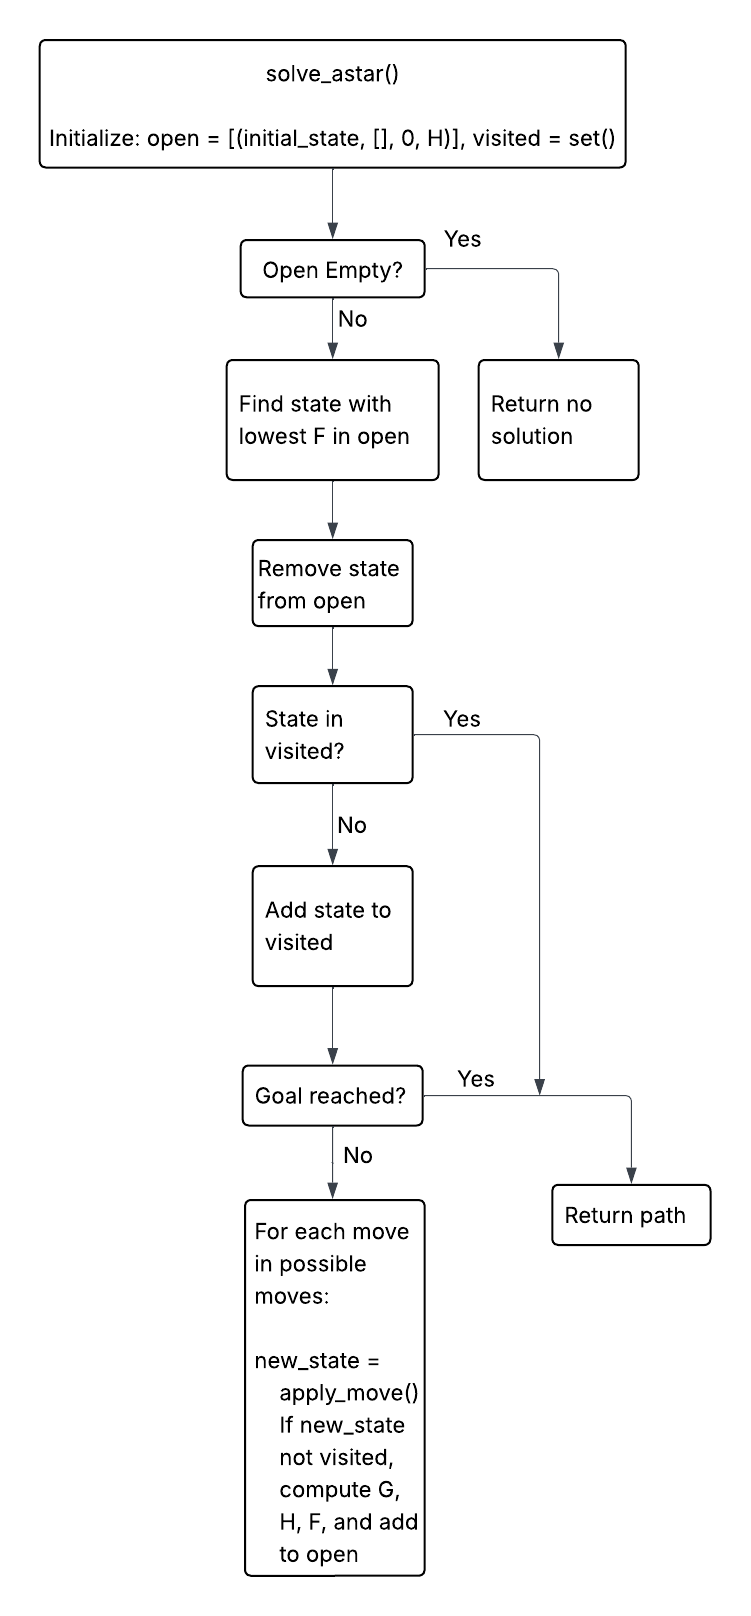
\includegraphics[width=0.6\linewidth]{pictures-Clarence/astar flowchart.png}
    \caption{Astar Flowchart Diagram}
    \label{fig:astar_flowchart}
  \end{figure}

\end{itemize}

\subsection{Tic-Tac-Toe Implementation(Full Code in Appendix)}

\begin{itemize}
  \item \texttt{BoardState Class} – Represents the game state with a 3x3 grid, tracks moves, and manages board operations.

  \item \texttt{apply\_move(row, col, is\_x)} – Places an 'X' or 'O' on the board at the specified position.

  \item \texttt{undo\_move(row, col)} – Reverts a move by clearing the specified position, essential for state exploration in Minimax.

  \item \texttt{get\_winner()} – Evaluates the board and returns the symbol of the winning player or None if no winner.

  \item \texttt{minmax()} – A recursive minimax algorithm that evaluates all possible moves to return a score for the current board state (-1, 0, 1).

  \item \texttt{minmax(alpha, beta)} – A recursive minimax algorithm with alpha–beta pruning, which evaluates possible moves more efficiently by pruning branches that cannot influence the final decision, while still returning a score for the current board state (-1, 0, 1).
\end{itemize}

\begin{figure}[H]
    \centering
    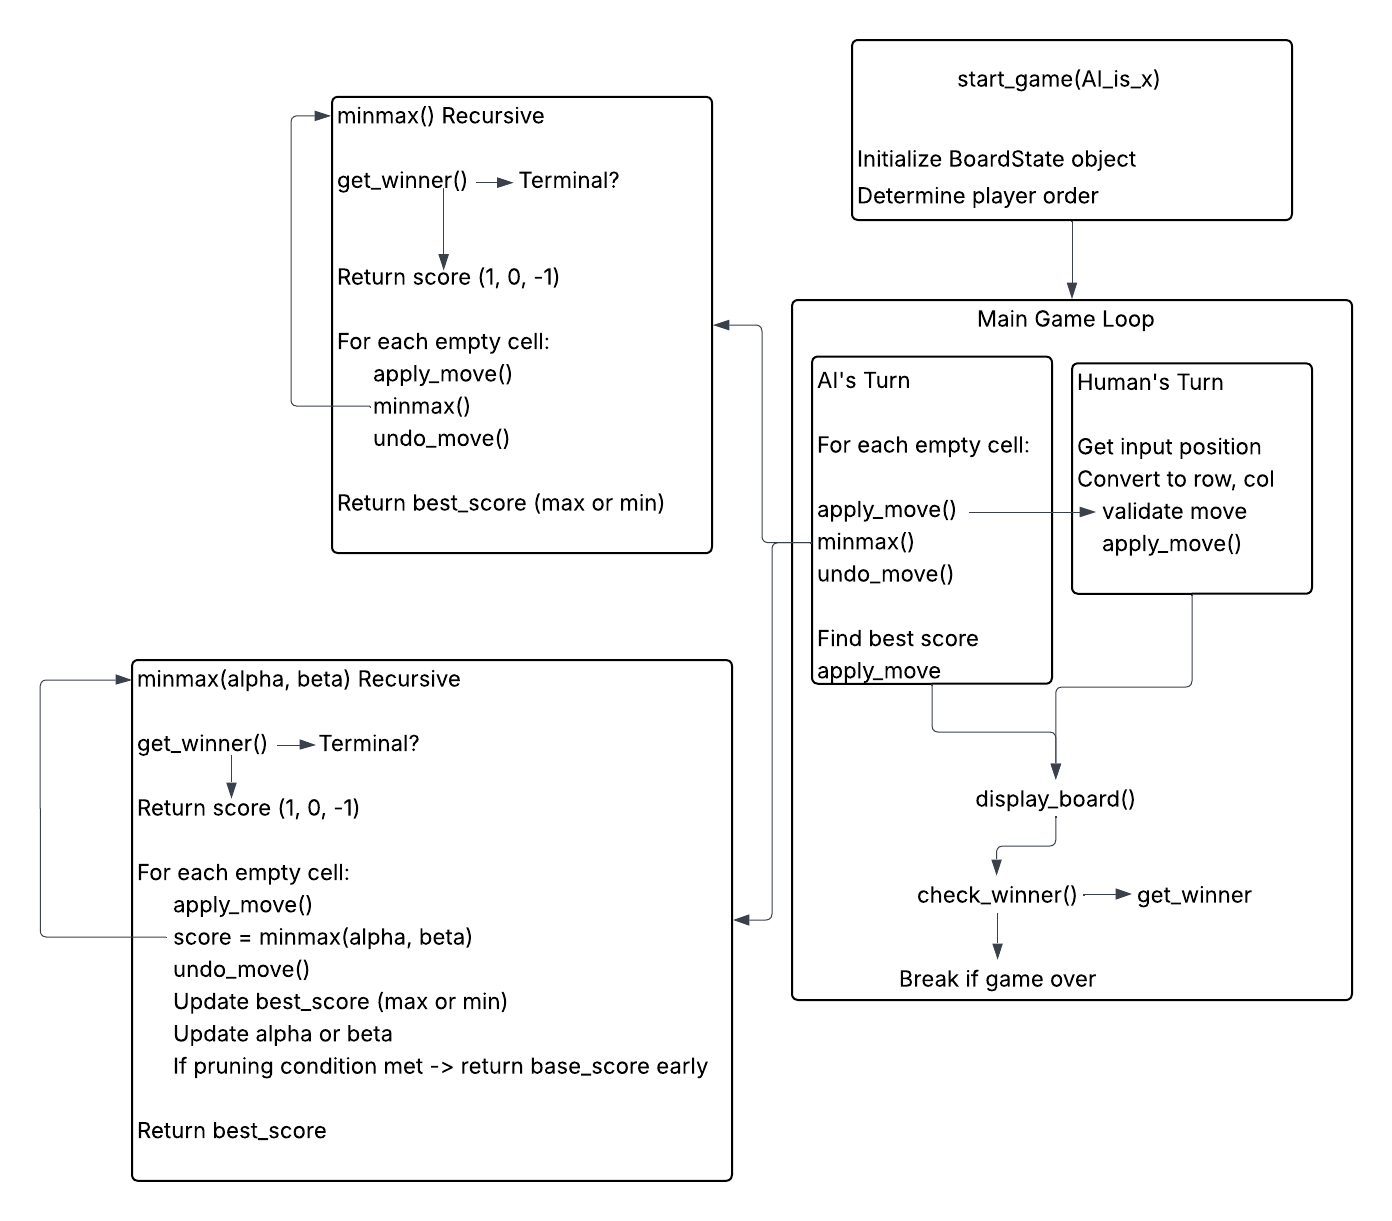
\includegraphics[width=0.6\linewidth]{pictures-Clarence/minmax flowchart.png}
    \caption{Minmax Flowchart Diagram}
    \label{fig:placeholder}
\end{figure}

\subsubsection{Choice of data structure, per algorithm, per exercise; and}
\subsubsection{What are the differences between each one’s implementation ?}
For the 8-puzzle solver, the uninformed search algorithms utilized distinct frontier management structures. Breadth-First Search employed a queue to guarantee that the shallowest, least-cost nodes were expanded first ensuring the shortest path at the cost of memory space. In contrast, Depth-First Search utilized a stack, prioritizing the deepest nodes in the current branch, which trades speed for reduced memory requirement per branch. The A* algorithm implemented the logic of a priority queue by maintaining an open list ordered by the sum F = G + H, where G is the path cost and H is the heuristic estimate. The node with the lowest F-cost was selected for expansion each iteration, guiding the search toward the goal.

For the adversarial Tic-Tac-Toe environment, the Minimax algorithm didn't use an external data structure for the frontier. Instead, its effectiveness derives from recursive state space exploration coupled with backtracking. The algorithm implicitly builds a game tree, leveraging the call stack to evaluate moves recursively. It employs a depth-first traversal to mark states with value -1 or 1 from terminal states back to the root, enabling the machine to select moves that maximize its advantage.
% SECTION 3
\section{Results}
\begin{figure}[H]
    \centering
    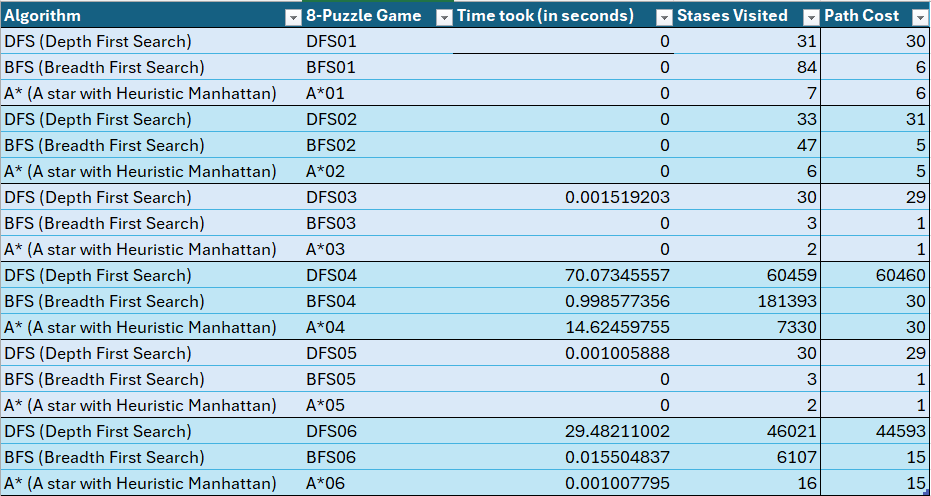
\includegraphics[width=1\linewidth]{pictures-Clarence/performance table.png}
    \caption{Performance Table Diagram}
    \label{fig:performance_table}
\end{figure}

The performance of the three algorithms was evaluated using six distinct test cases (see Appendix). 
Performance was assessed according to the following criteria:

\begin{itemize}
    \item \texttt{Execution time} – measured in seconds using Python's \texttt{time} module. Snapshots were recorded immediately before and after the algorithm’s execution, and the elapsed time was obtained by subtracting the start time from the end time.  
    \item \texttt{States visited} – determined by the number of unique board configurations explored, calculated as the final size of the \texttt{visited} set.  
    \item \texttt{Path cost} – defined as the length of the move sequence in the solution path.  
\end{itemize}

\subsection{Performance Evaluation}
\begin{figure}[H]
    \centering
    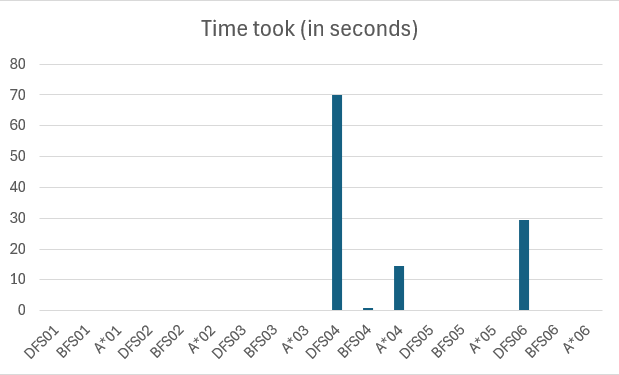
\includegraphics[width=1\linewidth]{pictures-Clarence/time took bar graph.png}
    \caption{Time took bar graph Diagram}
    \label{fig:time_bar_graph}
\end{figure}
The execution time of the algorithms varied depending on the initial board configuration. As shown in Figure~\ref{fig:time_bar_graph}, Test Case 1 was relatively straightforward for all algorithms, with near-instantaneous completion times (within the margin of computational precision, prone to truncation errors beyond the 11th decimal place). In contrast, Test Case 4 proved to be significantly more complex, particularly for the Depth-First Search (DFS) algorithm, which required approximately 70 seconds to reach a solution.  

Overall, the results confirm expected theoretical performance: the A* algorithm consistently outperformed the others in terms of efficiency, followed by Breadth-First Search (BFS), while Depth-First Search (DFS) exhibited the longest execution times.  

\begin{figure}[H]
    \centering
    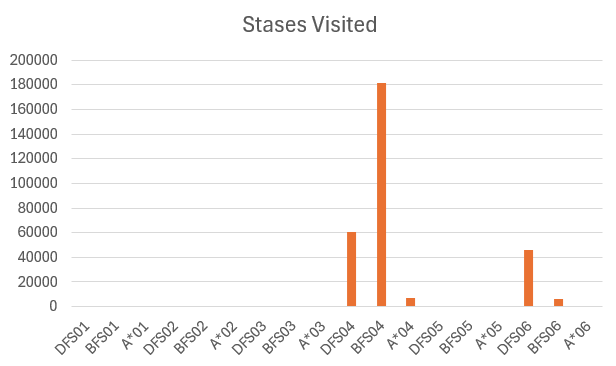
\includegraphics[width=1\linewidth]{pictures-Clarence/stases visited bar graph.png}
    \caption{States visited bar graph Diagram}
    \label{fig:stases_visited_bar_graph}
\end{figure}
The number of states visited exhibited similar variation patterns to execution time, as illustrated in Figure~\ref{fig:stases_visited_bar_graph}. The A* algorithm demonstrated superior efficiency in state exploration, visiting substantially fewer nodes than both BFS and DFS across all test cases. This efficiency stems from the heuristic guidance provided by the Manhattan distance metric, which effectively directs the search toward promising paths. BFS consistently visited an intermediate number of states, while DFS exhibited the least efficient exploration strategy, often expanding a large number of irrelevant nodes before finding the solution.

\begin{figure}[H]
    \centering
    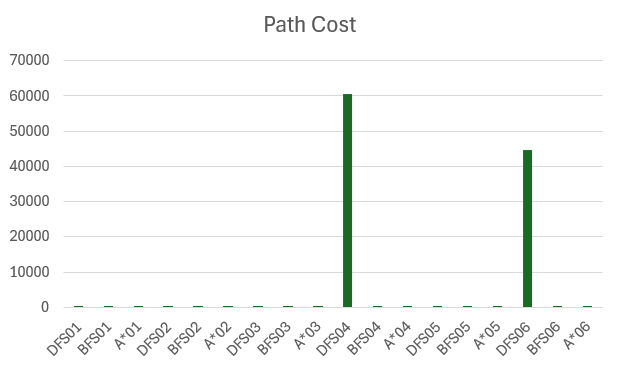
\includegraphics[width=1\linewidth]{pictures-Clarence/path cost bar graph.png}
    \caption{Path cost bar graph Diagram}
    \label{fig:path_cost_bar_graph}
\end{figure}
The solution quality, measured by path cost (number of moves required to reach the goal state), revealed significant differences between algorithms, as depicted in Figure~\ref{fig:path_cost_bar_graph}. Both A* and BFS consistently produced optimal solutions with minimal path lengths, confirming optimality for this problem domain. However, DFS frequently generated suboptimal solutions with substantially longer path lengths, particularly in more complex test cases. This behavior aligns with theoretical expectations, as DFS lacks mechanism for guaranteeing solution optimality and may explore deep, inefficient paths before finding a solution.

\subsection{Minimax}
When evaluating the performance of the minimax algorithm, two additional counters were introduced into the board state in order to measure efficiency. Since the majority of computation occurs during the initial move, these counters were designed to capture meaningful performance differences between the naive and optimized approaches. For both algorithms, a counter state.node count was used to track the total number of nodes explored. In addition, for the alpha–beta pruning variant, a second counter state.prune count was implemented to record the number of branches pruned during the search. The results of these measurements are presented below.

\subsection{Naive Minimax}
\begin{itemize}
    \item Nodes explored: 549946
    \item Execution time: 0.7795975208282471 seconds
\end{itemize}

\subsection{Minimax with Alpha-Beta}
\begin{itemize}
    \item Nodes explored: 21112
    \item Prunes: 4926
    \item Execution time: 0.03299546241760254 seconds
\end{itemize}
 
The results demonstrate the significant efficiency gains achieved through the use of alpha-beta pruning. Compared to the naive minimax algorithm, the pruned version explored much fewer nodes and achieved a noticeably faster execution time. This improvement is attributed to the pruning mechanism, which effectively eliminates branches that cannot influence the final outcome, increasing the speed without affecting correctness.

% SECTION 4
\section{Conclusion}
AI, in its most primal state, is the process of searching for solutions within a defined space. 
This search is completed through algorithms such as DFS, BFS, A*, and Minimax. While some 
algorithms generally outperform others, for instance, BFS typically explores fewer nodes than DFS, there 
exist problem instances where DFS may yield faster results. In the case of the 8-puzzle, A* 
demonstrated clear superiority, achieving the best balance of time and memory efficiency by using the
heuristic as a guide. For the tic-tac-toe game, Minimax with alpha–beta pruning consistently outperformed 
the naive Minimax approach, as pruning allows the algorithm to ignore branches that are non-beneficial.  

These findings highlight a central theme in artificial intelligence: the effectiveness of an algorithm 
is highly dependent on the nature of the problem being solved. Search methods that use 
heuristics or optimization strategies, such as A* and alpha–beta pruning, tend to scale better 
than their naive counterparts. Future work may extend these comparisons to larger state spaces or more 
complex games, further underscoring the trade-offs between time complexity,  and space complexity that lie 
at the core of AI problem-solving.

\subsection{Real-world Application of the AI algorithms}
Navigation in complex environments provides a clear real-world application of search algorithms. 
For example, consider the layout of a large shopping mall. To locate a particular store, one could 
apply depth-first search (DFS) or breadth-first search (BFS) to systematically explore paths within 
the mall until the goal is found. However, these approaches may be inefficient, as they do not take 
into account any knowledge of the mall’s layout. In contrast, the A* algorithm can be used to plan 
an optimal route by combining actual distances traveled with heuristic estimates of the remaining 
distance, allowing for faster and more efficient navigation.

\subsection{What did you learn or realize about “How AI works?”?}
I realized that many AI systems can be reduced to search processes. In games, enemy AI searches for 
the nearest player. In language models, the system searches for the most probable next word. In barcode scanners 
search for line patterns to convert into signals and more.  

\subsection{Future improvements of the AI algorithms}
For the first three algorithms, using object-oriented programming from the start would have improved 
modularity. A better hashing method could also replace the simulated one. In Minimax, the 
BoardState class could be redesigned to separate AI logic from the board state.  

\subsection{What did you learn or realize about “How AI should be used responsibly?”?}
Some fear AI will replace jobs, but history shows new technologies often create new opportunities. 
Like the steam engine, AI may replace certain roles, but those who adapt can use it to complement 
rather than compete with human labor.  

\subsection{Challenges of the AI algorithms}
In BFS and DFS, I mistakenly initialized the visited set with the initial state, which caused 
infinite loops. For Minimax, the main challenge was understanding its recursive structure, which 
seemed complex at first but became clearer with practice.  

\subsection{What did you learn or realize about “How AI is affecting society?”?}
Many people now rely on AI for convenience, sometimes at the cost of critical thinking. Over-reliance 
may lead to complacency, so AI should be used to enhance human ability rather than replace it.  

% SECTION 5
\section{Responsible Use of AI}

\subsubsection{How much AI did you use? }
None
\subsubsection{Justification for responsible use}
N/A
% APPENDICES
\appendix

\section{Additional Code Snippets}
\subsection{Test Cases Used in Evaluation}
The following test cases were utilized for algorithm performance evaluation as well as the code for the algorithms DFS, BFS, A*, and minmax are located within the github folder "exercise codes bernardino":

\url{https://github.com/Clarence Bernardino/bernardino_claveria_s1paper.git}


% BIBLIOGRAPHY
\bibliographystyle{IEEE/IEEEtran}
\bibliography{cs190-ieee}
% \nocite{*}

% BIOGRAPHY
\begin{biography}[{\includegraphics[width=1\linewidth]{pictures-Clarence/Profile Pic.png}}]{Clarence Joshua T. Bernardino} A Computer Science student at University of the Philippines Los Baños. Loves tinkering with code and Game of Thrones. Hopes to one day make a meaningful impact in the world by technology. 
\end{biography}

%%%%%%%%%%%%%%%%%%%%%%%%%%%%%%%%%%%%%%%%%%%%%%%%%%%%%%%%%%%%%%%%%%%%%%%%%%
% Elisha Julianne Claveria 

\newpage
\clearpage

\setcounter{section}{0}
\renewcommand{\thesection}{\Roman{section}}

%EXTENDED INTRODUCTION - Elisha
\stepcounter{section}
\section*{\normalsize \thesection. EXTENDED INTRODUCTION}
\addcontentsline{toc}{section}{\thesection. Extended Introduction}

\section{Extended Introduction}
Artificial Intelligence search algorithms such as Breadth-First-Search, Depth-First-Search, A*, 
and Minimax with Alpha-Beta-Pruning are essential in solving complex problems across various fields. 
These algorithms enable fast and efficient exploration of graphs or states which is immensely beneficial 
for pathfinding and decision-making type environments. Games such as the 8-puzzle and Tic-Tac-Toe are 
fitting examples of the implementation of these algorithms. This paper focuses on comparing the 
said algorithms through game implementations and performance analyzation. By evaluating the BFS, 
DFS, and A* uninformed and informed search and the Minimax with Alpha-Beta-Pruning adversarial search, 
we show each of their efficiency and limitations.


\subsection{Algorithmic comparison of BFS, DFS, A*, minimax}
What is your understanding of the algorithms based on the three exercises?

\subsection{Breadth-First Search (BFS) and Depth-First Search (DFS)}

The BFS and DFS are graph search algorithms that traverse through a graph or a collection of nodes. 
These two search algorithms use the data structures queue and stack respectively in assessing 
the best possible evaluation of such nodes. BFS and DFS also differ from each other due to 
their manner of searching wherein the BFS algorithm goes level-by-level. On the other hand, 
DFS starts from the “bottom” or the newly inserted nodes of the graph.\cite{puppyGraph-Graph-Search-Algorithms} 

\subsection{A* Search}
The A* search is also a search algorithm that has a different approach to reach the goal, 
the best possible path/s to get to the evaluated or “goal” node in a graph. 
It uses an evaluation function that utilizes the cost of the path taken by taking in the distance traveled (g(n)) 
and the estimated remaining distance, also known as the heuristic function(h(n)). Adding these together we get f(n) which 
results into the most optimal node that balances the cost and remaining distances.

\subsection{Minimax Search}
The Minimax Search is essentially a game algorithm whose given always behave optimally and a 
player who attempts to maximize their chances of winning by assuming the opponent is playing 
optimally. This algorithm checks and evaluates all possible moves in a game tree that can be 
made through a recursive algorithm. It considers the possible moves the maximizing player can make 
and chooses one that practically maximizes the other player’s worst move or outcome.


\setcounter{section}{1}
\renewcommand{\thesection}{\Roman{section}}

\stepcounter{section}
\section*{\normalsize \thesection. EXTENDED METHODS}
\addcontentsline{toc}{section}{\thesection. Extended Methods}


% SECTION 2
\section{Extended Methods}
For the 8-puzzle implementation, a dictionary was primarily used to map integers from 1 to 9 to another 
set of integers from 0 to 8, representing the slots or tiles of the game board. Additionally, other data 
structures such as lists, queues, and stacks were employed in the implementation of the search algorithm functions.
For the Tic-Tac-Toe implementation, a dictionary was used to map integers from 1 to 9 to 
either ``\_’’, ``X’’, or ``O’’. This structure efficiently updates and accesses board positions throughout the game.

\subsection{8-puzzle Implementation (Full Code in Appendix)}
\begin{itemize}
  \item \texttt{empty\_slot(board)} – takes in the puzzle board and finds the position or index of the empty slot(‘0’) in the board.

  \item \texttt{valid\_moves(i)} – takes (‘i’) position and checks for all its possible moves. It returns a list of the tile at position (‘i’) with its adjacent positions.

  \item \texttt{move(board, pos)} – takes in the puzzle board and the pos (empty slot) and moves it based on the user’s input of (‘w’ (up), ‘a’ (left), ‘x’ (down), ‘d’ (right). It then calculates for the new position.

  \item \texttt{check\_win(board)} – takes in the puzzle board and checks if it matches with the goal state.

  \item \texttt{solve\_bfs(initial\_state)} – solves the puzzle board using Breadth-First-Search which finds the shortest path to reach the goal state.

  \item \texttt{solve\_dfs(initial\_state)} – solves the puzzle board using Depth-First-Search which explores each branch of the graph until reaching the goal state.

  \item \texttt{heuristic(initial\_state)} – calculates for the number of misplaced tiles in comparison to the supposed goal state for the puzzle.

  \item \texttt{solve\_astar(initial\_state, heuristic)} – implements the A* search algorithm and finds the shortest path from the initial to goal state, utilizing the heuristic function. 
\end{itemize}

\subsection{Tic-tac-toe Implementation (Full Code in Appendix)}
\begin{itemize}
  \item \texttt{check\_win(spaces)} – takes in the game board(spaces) and checks for all the possible winning combinations on the board (rows, columns, or diagonals). It then checks for a winner.

  \item \texttt{utility(spaces)} – takes in and evaluates the game board for the minimax algorithm. It assigns a resulting value or score based on the result.

  \item \texttt{max\_value(spaces, a, b)} –  recursive function that simulates the moves to find the maximum utility for the maximizing player.

  \item \texttt{min\_value(spaces, a, b)} – recursive function that simulates the moves to find the minimum utility for the minimizer player.

  \item \texttt{alpha\_beta\_search(spaces, player)} – utilizes minimax algorithm with alpha-beta pruning to find the best possible move for the player.
\end{itemize}


\subsubsection{Choice of data structure, per algorithm, per exercise; and}
\subsubsection{What are the differences between each one’s implementation ?}.\newline
The 8-puzzle game used uninformed and informed search algorithms for state exploration. 
Breadth-First-Search used a queue, to find the shortest possible solution path. On the other hand, 
Depth-First-Search used a stack to explore each branch up to the last nodes of the graph. The A* algorithm 
utilized a heuristic function for counting misplaced tiles. Given this, it uses an evaluation function 
of F = G(path cost) + H (heuristic value). This balances the performance of the player, being the most optimal.

The Tic-tac-toe game, used an adversarial search utilizing the Minimax algorithm 
together with alpha-beta pruning. The code implements utility evaluation and searches through possible 
moves recursively and finds the most optimal move for the maximizing player. Comparing this to the 8-puzzle 
game, instead of searching for a single fixed goal, the former is concerned with making decisions  against an 
opponent. Entailing maximizing and minimizing the moves until an end result.


\setcounter{section}{2}
\renewcommand{\thesection}{\Roman{section}}

\stepcounter{section}
\section*{\normalsize \thesection. EXTENDED RESULTS}
\addcontentsline{toc}{section}{\thesection. Extended Results}


% SECTION 3
\setcounter{section}{2}
\renewcommand{\thesection}{\Roman{section}}

\stepcounter{section}
\section*{\normalsize \thesection. EXTENDED RESULTS}
\addcontentsline{toc}{section}{\thesection. Extended Results}


\section{Extended Results}

\setcounter{figure}{0}
\begin{figure}[H]
    \centering
    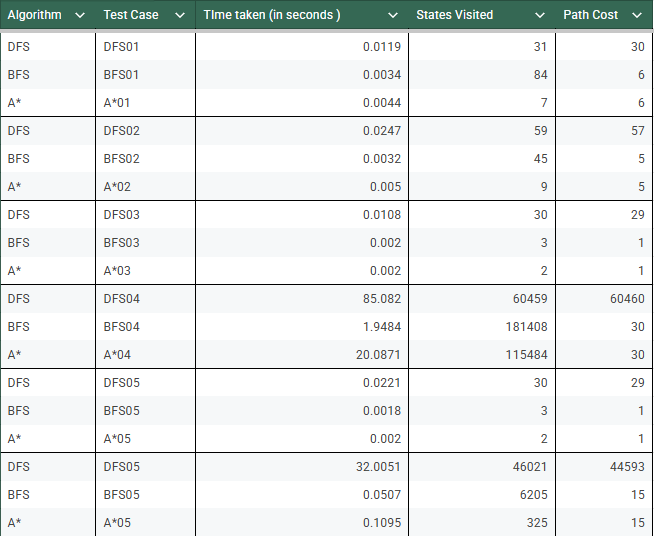
\includegraphics[width=0.8\linewidth]{pictures-Elisha/results_table.PNG}
    \caption{Performance Table Diagram}
    \label{fig:performance_table}
\end{figure}

The table shows a detailed  breakdown of time taken (in seconds), states visited, and path cost for each 
algorithm (DFS, BFS, A Star*) across the test cases(1-6), offering precise numerical insights. It confirms 
the trends seen in the charts, with A04 and A05 showing the highest values across all metrics. 

The performance of the three algorithms was evaluated using six distinct test cases (see Appendix). 
Performance was assessed according to the following criteria:

\begin{itemize}
    \item \texttt{Execution time} – measured in seconds using Python's \texttt{time} module. Snapshots were recorded immediately before and after the algorithm’s execution, and the elapsed time was obtained by subtracting the start time from the end time.  
    \item \texttt{States visited} – determined by the number of unique board configurations explored, calculated as the final size of the \texttt{visited} set.  
    \item \texttt{Path cost} – defined as the length of the move sequence in the solution path.  
\end{itemize}

\subsection{Performance Evaluation}
\begin{figure}[H]
    \centering
    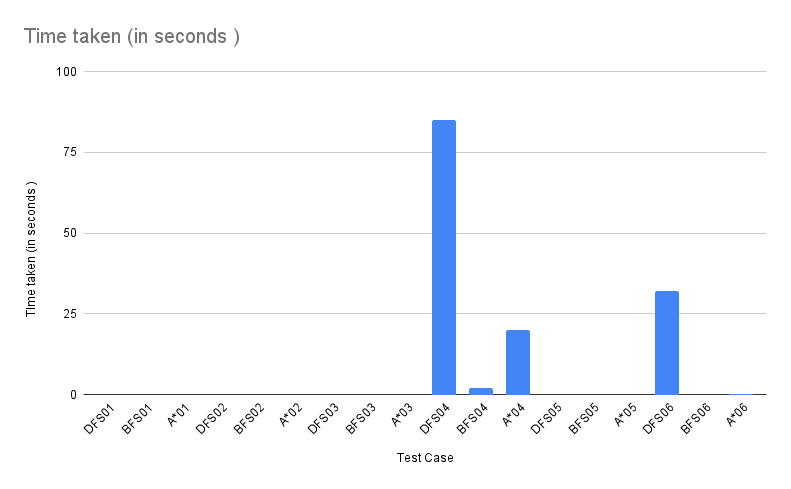
\includegraphics[width=1\linewidth]{pictures-Elisha/Time taken (in seconds ).png}
    \caption{Time taken bar graph Diagram}
    \label{fig:time_bar_graph}
\end{figure}

The table shows the time measurements for each algorithm and its test case. Most of which are fast or 
rapid as compared to other test cases having most values near 0. On the other hand, Test Case 4 for the 
DFS (around 85 seconds) and A Star Algorithm (around 20 seconds), and Test Case 6  for the DFS Algorithm (around 32 seconds), 
showing substantial execution time for these three instances. Based on these results, It illustrates how the Depth-First 
Search algorithm is more time-intensive compared to the other two search algorithms. Also, It shows how the 
different test cases affect execution time, wherein Test Cases 4 and 6 appear to be more complicated than of the others. 

All in all, the A star algorithm appears to be the most efficient search algorithm, based on execution 
time, compared to the BFS and DFS search algorithms.

\begin{figure}[H]
    \centering
    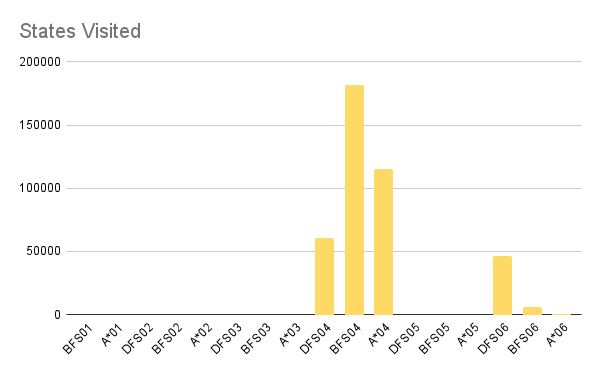
\includegraphics[width=1\linewidth]{pictures-Elisha/States Visited (1).png}
    \caption{States Visited bar graph Diagram}
    \label{fig:states_visited_bar_graph}
\end{figure}

As seen in this chart, It shows the number of states visited across all the test cases. 
It is evident in Test Cases 4 and 6 there is a significant difference among the other cases. 
Test Case 4 using BFS Algorithm shows the highest number of states. It stays consistent how Test Case 
4 appears to be the more complex case among the rest. Similarly, A star Algorithm also stays 
consistent as the most efficient algorithm.

\begin{figure}[H]
    \centering
    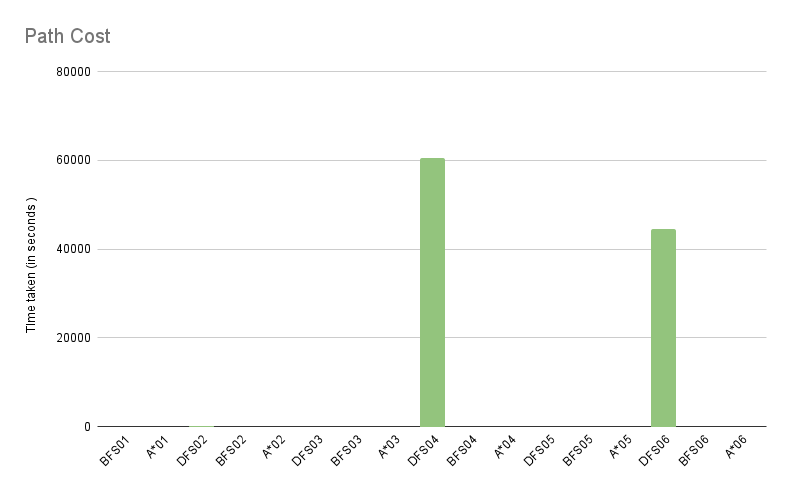
\includegraphics[width=1\linewidth]{pictures-Elisha/Path Cost (1).png}
    \caption{Path Cost bar graph Diagram}
    \label{fig:path_cost_bar_graph}
\end{figure}

The chart shows the path cost with most Test Cases showing minimal time except again for 
Test Cases 4 and 6, peaking at around 60,000 and 40,000 respectively. Additionally, the chart 
shows significant results for the BFS and A Star search algorithms once again. Such results stay 
consistent with the previous findings, overall, the A star algorithm appears to be the most efficient 
and optimal search algorithm.


\subsection{Minimax}

\subsection{Naive Minimax}
\begin{itemize}
    \item Nodes explored: 15172
    \item Execution time:  0.042225 seconds
\end{itemize}

\subsection{Minimax with Alpha-Beta}
\begin{itemize}
    \item Nodes explored: 1086
    \item Prunes: 410
    \item Execution time: 0.004222 seconds
\end{itemize} 


Based on these results, the Alpha-Beta-Pruning Algorithm outperformed the Naive Minimax 
Algorithm having an average execution time of 0.004222 seconds making it around 10 times faster 
than the latter. Additionally, the nodes explored by the Alpha-Beta-Pruning Algorithm have fewer 
than Naive Minimax, due to the pruning mechanism utilized. Overall, the results show the efficiency 
of Alpha-Beta-Pruning Algorithm in making optimal moves as well as reducing search spaces.


% SECTION 4
\setcounter{section}{3}
\renewcommand{\thesection}{\Roman{section}}

\stepcounter{section}
\section*{\normalsize \thesection. EXTENDED CONCLUSION}
\addcontentsline{toc}{section}{\thesection. Extended Conclusion}

\section{Extended Conclusion}
In essence, this study shows a comprehensive understanding of various search algorithms 
through their utilization in the games: 8 puzzle and Tic-Tac-Toe. The study emphasizes the 
differences of such algorithms showing how they work differently. Breadth-First-Search and 
Depth-First-Search are Uninformed Search Strategies which involve traversing through graphs 
using queues and stacks. The A star is an Informed Search Strategy algorithm which utilizes 
heuristics and lastly the Minimax Alpha-Beta-Pruning Algorithm is an Adversarial Search or Decision Making. 

Overall, the results show A Star Algorithm as the most efficient for solving the 8-puzzle 
game which consistently outperformed the BFS and DFS Algorithms in terms of Execution Time, 
States Visited, and Path Cost. Moreover, In the Adversarial Search Algorithms, the Alpha-Beta-Pruning 
proves to be more optimal than the naive Minimax. This is seen in the results wherein the former had an 
approximately 10 times faster execution than the latter, exploring lesser nodes, and having an average of 
410.50 prunes. All in all, these findings indicate the value of heuristics and pruning in further enhancing 
efficiently and optimality.

\subsection{Real-world Application of the AI algorithms}
The Breadth-First-Search (BFS), Depth-First-Search (DFS), and A* algorithms can be utilized in
path-finding problems such as in games, navigation, and route planning. Additionally, the
Minimax and Alpha-Beta-Pruning algorithms can be applied to game engines, decision-making, and in models.

\subsection{Future Improvements of the AI algorithms}
For the 8-puzzle game, I could have improved the AI Algorithm through the use of a better 
heuristic function such as the Manhattan Distance. Additionally, for both game implementation, 
a better representation for the boards or states could have improved the optimization and 
efficiency of these algorithms.

\subsection{Challenges of the AI algorithms}
With the past three exercises, I had most difficulty with the Depth-First-Search Algorithm as well as the 
A Star Algorithm. Since I had to finish the exercises only within lab hours I struggled to make my work 
fully working and optimized. I was able to fully grasp and finish my code, only after my laboratory class. 
This shows how I need to put more effort into understanding the implementation of AI algorithms and in optimizing my time.

\subsection{What did you learn or realize about “How AI works?”?}
With the past three exercises, I learned how AI, as seen in the 8-puzzle game and Tic-Tac-Toe, works by 
utilizing algorithms such as the BFS, DFS, A*, and Minimax in order to evaluate states through search and 
optimization mechanisms or strategies. I realized how AI can not only provide optimal solutions to simple 
game problems, but also to other real-world problems. By analyzing models, optimizing logistics, and searching for 
patterns, Artificial Intelligence’s reach extends to varying applications further enhancing efficiency in many 
industries such as transportation, technology, and healthcare.

\subsection{“How it should be used responsibly?”}
AI should be used with transparency, Its use should be first acknowledged. The users of 
Artificial Intelligence should also be accountable for whatever consequences AI's use may carry. 
Moreover, to responsibly use AI is to use it for good and not for any deceitful endeavors.

\subsection{“How it is affecting society?”}
As a Computer Science student, I believe that AI has overall impacted our growth and 
development by enhancing various industries in, as mentioned before, transportation, 
technology, and healthcare. While Artificial Intelligence has quickly aided optimization 
and improvements in our society, there is still an issue in its way of ethical use. Given 
this, using AI should always be guided with transparency, accountability, and integrity.

%SECTION 5
\setcounter{section}{4}
\renewcommand{\thesection}{\Roman{section}}

\stepcounter{section}
\section*{\normalsize \thesection. EXTENDED RESPONSIBLE USE OF AI}
\addcontentsline{toc}{section}{\thesection. Extended Responsible Use of AI}

\section{Extended Responsible Use of AI}

\subsection{How much AI did you use in your work, which parts of your work involved the use of AI tools?}
I used AI tools in my base code for the 8-puzzle problem. I specifically utilized AI tools in my move(board, pos) function.

\subsection{Explain how you used AI responsibly and ethically in completing the task.}
Since I was having a difficult time in fully grasping the logic for the possible moves the user can do, 
I inquired on how I can get the value of the new position (when the current position is swapped onto the next) 
and I applied the logic through mathematics, since I already have the values for the row and column of the 0 or 
empty slot.

% APPENDICES
\appendix

\section{Additional Code Snippets}
\subsection{Test Cases Used in Evaluation}
The following test cases were utilized for algorithm performance evaluation as well as the code for the algorithms DFS, BFS, A*, and minmax are located within the github folder "exercise codes bernardino" and "exercise codes claveria":

\url{https://github.com/Clarence Bernardino/bernardino_claveria_s1paper.git}


% BIBLIOGRAPHY
\bibliographystyle{IEEE/IEEEtran}
\bibliography{cs190-ieee}
% \nocite{*}


% BIOGRAPHY
\begin{biography}[{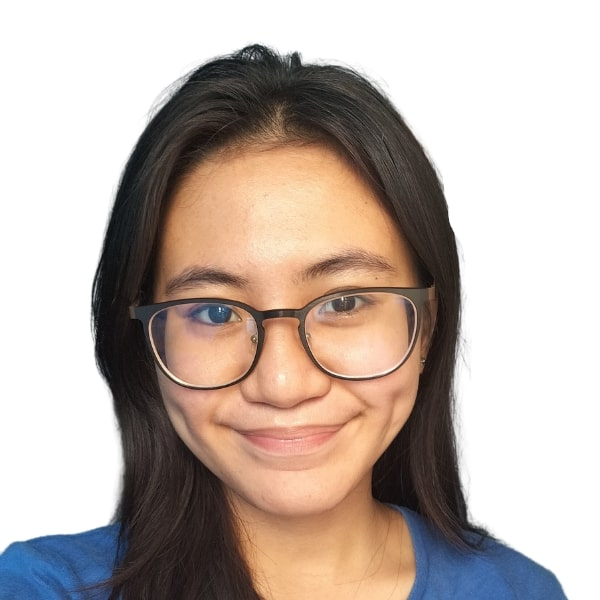
\includegraphics[width=1\linewidth]{pictures-Elisha/Claveria_2x2.jpg}}]{Elisha Julianne V. Claveria} 3rd year Bachelor of Science in Computer Science at University of the Philippines. Enjoys creating art, mainly through paintings and sketches.  
\end{biography}

\end{document}